\section{Experiment Design}\label{sec:experiment_design}
%Forsoegsopstilling, der inkludere en tegning af omraadet set oppefra med indtegning af beacons, objectern og hvor rigtige position for test person.
We conducted experiments in a room measuring $4.75m \times 6.5m$ to evaluate the implemented system described in Chapter~\ref{chap:system_design}.
In the room, a cabinet is placed between two tables, effectively dividing the room into two smaller areas. 
Each of the smaller areas are furnished with a table surrounded by six chairs, and whiteboards mounted on the walls.

On one end of each table is a large, rectangular window.
Furthermore, one table has a large TV screen placed near its window. 
Near the door of the room, an airconditioning controller and a large glass pane, acting as a window out into the common area, is located. 
Next to the door is placed a glass pane, acting as a window out into the common area. 
Lighting is built into the ceiling, thus no hanging light will interfere with the broadcasted signals. 
Outside the meeting room, is the aforementioned common area containing two high tables.
Each of these tables has a small couch and two chairs placed next to it.
The meeting room and its surrounding area are depicted in Figure \ref{fig:experiment_room}.
The room was provided as-is by AAU, so using it provides a realistic setting for experimentation.

To create the map, the room and the common area was partitioned into a $1m \times 1m$ grid using painter's tape.
Measurements for the map were taken where gridlines intersect.
This resulted in $6 \times 4$ measurements with a classification label of \textit{inside} being taken inside the room.
The common area outside of the room was partitioned in the same fashion, resulting in  $6 \times 2$ classification labels of \textit{outside}. 


\begin{figure}
    \centering
    \begin{subfigure}[b]{0.48\textwidth}
        \centering
        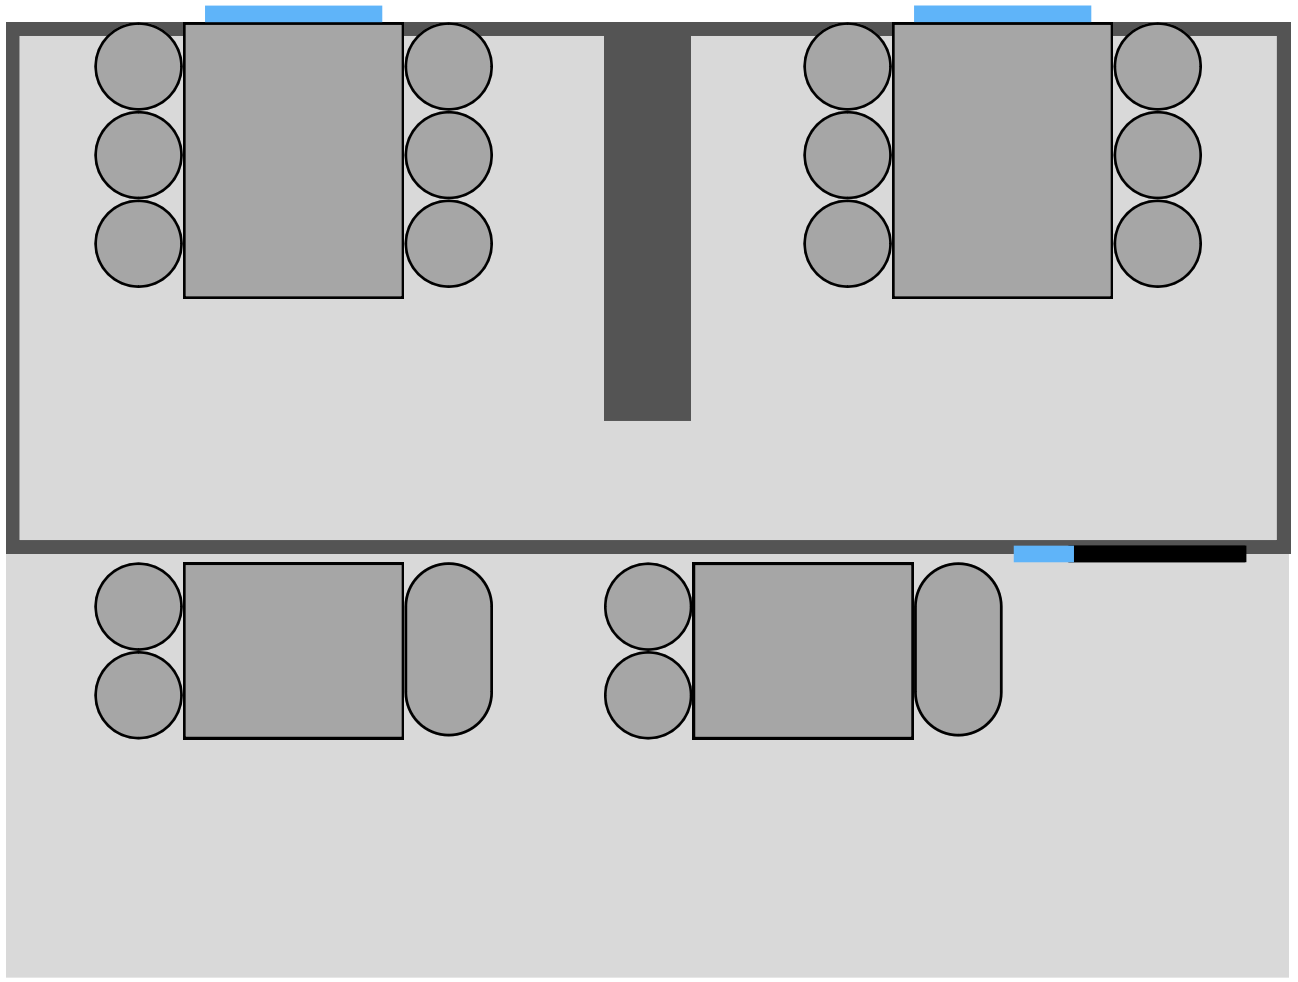
\includegraphics[width=\textwidth]{images/experiment_room.png}
        \caption{A sketch showing the room and the common area in which the experiments take place.}
        \label{fig:experiment_room}
    \end{subfigure}
    \begin{subfigure}[b]{0.48\textwidth}
        \centering
        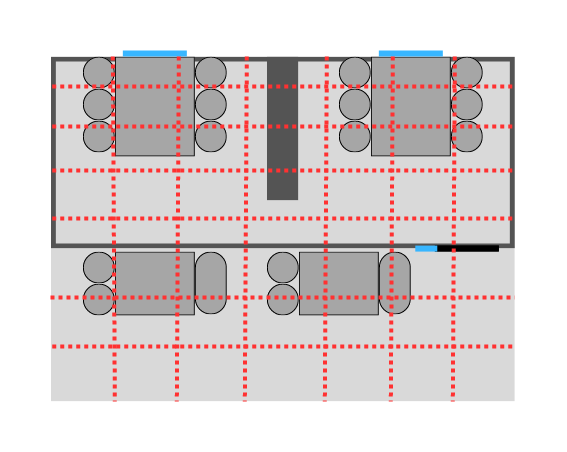
\includegraphics[width=\textwidth]{images/roomwithgrid.png}
        \caption{The gridwise partition of the experiment room and the common area (red).}
        \label{fig:room_partition}
    \end{subfigure}
    \begin{subfigure}[b]{0.48\textwidth}
        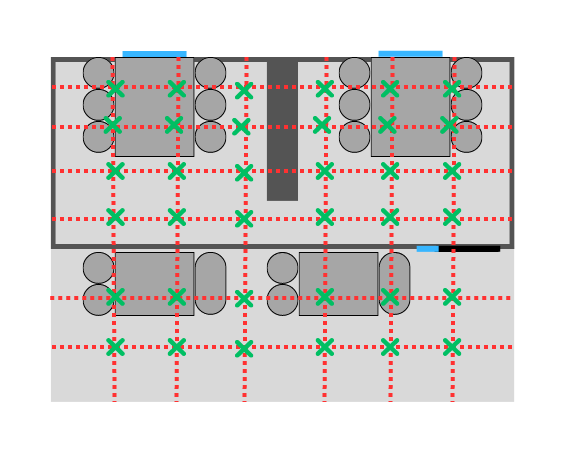
\includegraphics[width=\textwidth]{images/roomwithgridandmeasurements.png}
        \caption{The partitioned room decorated with locations where measurements are taken (green).}
        \label{fig:room_partition_measurements}
    \end{subfigure}
    \begin{subfigure}[b]{0.48\textwidth}
        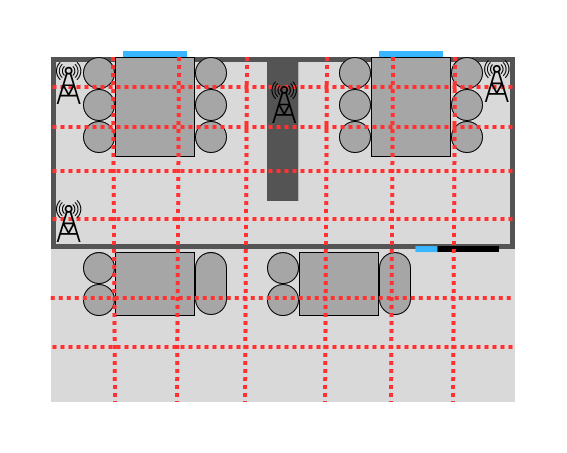
\includegraphics[width=\textwidth]{images/gridwithbeacons.png}
        \caption{The partitioned room with four iBeacon BLE9 Bluetooth beacons.}
        \label{fig:room_partition_beacons}
    \end{subfigure}
    \caption{The room and common area in which the experiment takes place. Figures \ref{fig:room_partition} and \ref{fig:room_partition_measurements} shows how the area is partitioned and where measurements are taken. Figure \ref{fig:room_partition_beacons} shows the placement of beacons when performing the experiments.}
    \label{fig:allfiguresForTheGridPartition}
\end{figure}
The gridwise partition of the room and the common area is shown in Figure \ref{fig:room_partition}, while Figure \ref{fig:room_partition_measurements} depicts the \textit{collection points} where measurements for the map were taken.
During the creation of the map, measurements were collected for each collection point until a standard deviation of under $6.5$dBm is achieved, with a minimum of $40$ measurements being required, as described in Section \ref{sec:data_collection_implementation}.
The map creation process was done during out-of-office hours to ensure that the datapoint collected to create the map was collected with a minimum of background signal noise.

During both the creation of the map and the classification, four iBeacon BLE9 Bluetooth beacons \cite{BluetoothiBeaconBLE9} were placed on top of the cabinet and in the three corners furthest away from the door. This is depicted on Figure \ref{fig:room_partition_beacons}.
The beacons in the corners of the room were placed at a height of $2.5m$, while the center beacon on top of the cabinet was placed at a height of $1.5m$.
The beacons placed near the windows were located on top of a whiteboard, while the beacon in the lower left corner of the room was held in place using painter's tape.

If one were to place a beacon close to the door of the meeting room, one makes the classification system dependent on a high precision.
This can be understood by imagining a scenario where a person is located in a position only just inside the meeting room.
By having a beacon by door, we risk that a slight fluctuation in the received signal strength from the beacon will result in the determined location being immediatedly outside the room (see Figure \ref{fig:room_partition_measurements}).
For this particular system, we would rather have classifications biased towards being inside of the room as to not cancel meetings that are ongoing, and therefore place beacons further inside the room.